\documentclass[a4paper]{IEEEtran}

% Ein paar hilfreiche Pakete
\usepackage[utf8]{inputenc}
\usepackage[ngerman]{babel}
\usepackage{graphicx}
\usepackage{caption}
\usepackage{subcaption}
\usepackage{amsmath}
\usepackage{amssymb}
\usepackage{mathtools}
%\usepackage[section]{placeins}
\usepackage{hyperref}
\usepackage{algpseudocode}
\usepackage{algorithm}

% Nummeriere Formel nur, wenn sie auch referenziert wird
\mathtoolsset{showonlyrefs}

% Für Code-Schnipsel
\def\code#1{\texttt{#1}}

% Für Pseudocode input und output einer funktion
\algblock{Input}{EndInput}
\algnotext{EndInput}
\algblock{Output}{EndOutput}
\algnotext{EndOutput}
\newcommand{\Desc}[2]{\State \makebox[3em][l]{#1}#2}

% Graphics Paths
\input
\graphicspath{{../../Media}}

% Für subfigure plots
\captionsetup[subfigure]{justification=centering}

% Header
\markboth{Proseminar Anthropomatik WS 21/22: Von der Theorie zur Anwendung}{Proseminar Anthropomatik WS 21/22: Von der Theorie zur Anwendung}

% Hier den Titel des eigenen Seminars eintragen
\title{Punkt-Warping: Inversionsmethode mit Hash-Tabelle}

% Hier deinen eigenen Namen
\author{Lukas Knirsch}

% --- START OF DOCUMENT ---
\begin{document}

% Erzeugt die Überschrift
\maketitle

% Abstract
\begin{abstract}
Bei wissenschaftlichen Simulationen oder bei hochqualitativen Schätzberechnungen werden sehr große Datensätze benötigt, 
die nach bestimmten Merkmalen verteilt sind \cite{frisch_hanebeck-deterministic_gaussian_sampling-2021}. Diese Daten können häufig durch Funktionen wie eine Normalverteilung oder 
multivariante Gaussche Verteilungen beschrieben werden. Umso gleichmäßiger die Daten aber verteilt sind, umso genauer  
können die Simulationen oder Schätzungen berechnet werden. Die dafür bereits verwendeten Methoden besitzen aber Nachteile, 
einer davon ist der hohe Rechenaufwand für die ungefähr gleichmäßige Verteilung im Raum. Aus diesem Grund soll in dieser 
Ausarbeitung die Funktionsweise und eine Implementation der hash-basierten Inversionsmethode erarbeitet werden und ihr 
möglicher Einsatz bei der gleichmäßigen Verteilung von Daten und Punkt-Warping im Allgemeinen.
\end{abstract}

% Text
\section{Einleitung}

In dieser Ausarbeitung soll eine Methode beschrieben werden, mit deren Hilfe man durch endlich viele Zufallszahlen 
eine ungefähr gleichmäßige Verteilung von Punkten im Raum generieren kann. Damit kann man sehr gut Daten simulieren, 
welche eine bestimmte Verteilung besitzen und, wie in der Natur üblich, keine harten Kanten besitzen oder komplett 
zufällig verteilt sind, sondern abfallen. Zu diesen Dichteverteilungen gehört zum Beispiel auch die Gaußschen Normalverteilung. 

Für die randomisierten Eingaben werden sogenannte "Golden Ratio Sequences", die von Schretter 
\cite{schretter-golden_ratio_sequences-2012} vorgestellt wurden, verwendet. Diese Punkte werden auf die von Chen 
und Asau \cite{chen_asau-generating_random_variates-1974} und Devroye \cite{devroye-non_uniform_random_variate-1986} 
beschriebene, verbesserte \hyperref[funktion]{Inversionsmethode} mit Hashing angewandt, wodurch das gewünschte Ergebnis 
erzielt wird. Diese Verfahrenskette wird unter \hyperref[impl]{Implementation} näher erläutert und durchgeführt. 


\subsection{Problemstellung}
Durch diese Ausarbeitung soll geklärt werden, wie die Hash-basierte Inversionsmethode funktioniert und ob  
sie bei der Generierung von multivariaten Verteilungen in höheren Dimensionen mithilfe von uniformen Dichten immer noch 
korrekt arbeitet und einsetzbar ist. Außerdem soll verglichen werden, ob sich der Einsatz der hier beschriebenen 
Methode als Ersatz von bereits existierenden anderen Methoden lohnt.

\begin{figure}
    \centering
    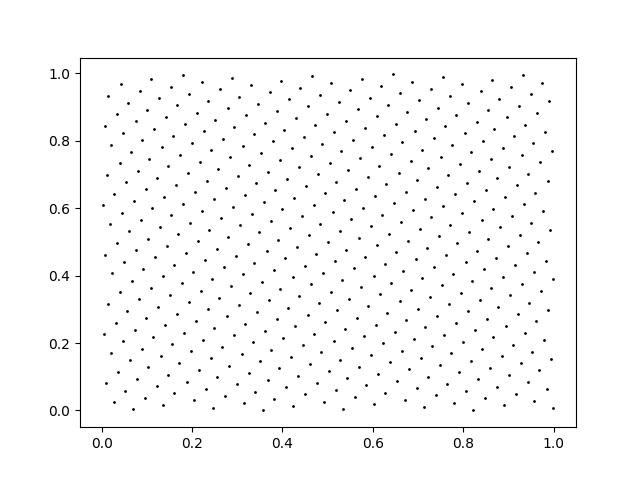
\includegraphics[width=0.48\textwidth]{grs_u500c.png}
    \caption{500 gleichmäßige, zufällige Punkte einer Goldenen-Schnitt-Sequenz \cite{schretter-golden_ratio_sequences-2012}.}
\end{figure}

\subsection{Stand der Technik}
Anstelle der hash-basierten Inversionsmethode kann auch ein Feld der Partialsummen der einzelnen Wahrscheinlichkeiten 
der zu generierenden Punkte verwendet werden. Auf dem Feld können dann unterschiedliche Methoden zum Finden der Werte 
verwendet werden. Dazu gehören lineare Suche von vorne nach hinten, binäre Suche oder ein Huffman-Baum.

Zur Generierung uniformer Zufallszahlen gibt es anstelle der Sequenzen des goldenen Schnittes auch Methoden wie
die von Halton \cite{wong_luk_heng-halton_points_sampling-1997}, Blue Noise \cite{yan-blue_noise_sampling-2015} oder Rang-1-Gitter 
\cite{prasad-rank1lattice-1973}. Doch da Schretter in seinem Paper zeigt, dass die von diesen Methoden generierten Zahlen 
nicht so gleichmäßig verteilt generiert werden, wie seine Vorgestellte \cite{schretter-golden_ratio_sequences-2012}, 
wird jene verwendet. 

\section{Funktionsweise}
\label{funktion}

Dieser Abschnitt erklärt die Arbeitsweise der Inversionsmethode im Allgemeinen. Danach wird kurz das Prinzip 
der Hashtabelle wiederholt, um danach die Funktionsweise der hash-basierten Inversionsmethode zu erläutern.


\subsection{Inversionsmethode}
Devroye \cite{devroye-non_uniform_random_variate-1986} beschreibt in seinem Buch die Inversionsmethode als eine 
Methode, bei der mithilfe des Inversen $F^{-1}$ einer bekannten Verteilungsfunktion $F$ und mit einer uniformen, 
zufälligen Zahl $U \in [0, 1]$ eine zufällige Zahl $X = F^{-1}(U)$ generiert wird. Dadurch gibt es eine monotone 
Beziehung zwischen $U$ und $X$, weshalb ein Paar $(x_1, x_2)$, bei dem $X_1$ und $X_2$ maximal anti-korreliert 
zueinander sind, mit 
\begin{equation}
    (F^{-1}(U),\, F^{-1}(1 - U))
\end{equation}
berechnet werden kann. Diese Eigenschaft wird vor allem in 
Simulationen benötigt.

Durch die Erzeugung der Zufallsvariable $X$ durch das Inverse einer Verteilungsfunktion kann die Inversionsmethode 
allerdings nur dann optimal angewandt werden, wenn $F^{-1}$ einfach zu berechnen ist oder sogar schon bekannt ist. 
Durch heutige numerische Algorithmen können aber auch Funktionen, welche nicht \glqq per Hand\grqq{} invertierbar sind, in der 
vorgestellten Weise benutzt werden. 

\begin{table}
    \centering
    \begin{tabular}{lll}
    Name         & Funktion & Zufällige Variable \\
                 &          &                    \\
    Exponentiell & $1 - e^{-x}$ & $\log(1/U)$ \\
    Logistisch   & $1 / (1 + e^{-x})$ & $-\log(\dfrac{1-U}{U})$ \\
    Cauchy       & $1/2 + (1/\pi) \arctan(x)$ & $\tan(\pi U)$
    \end{tabular}
    \caption{Explizit invertierbare Verteilungsfunktionen \cite{devroye-non_uniform_random_variate-1986}}
    \label{fig:invFuncs}
\end{table}

Nach Devroye können, nur unter Verwendung sogenannter \glqq einfachen Transformationen\grqq, Paare von unabhängigen 
Variablen generiert werden. Zum Beispiel kann mit der Standardnormalverteilung $\dfrac{e^{-x^2/2}}{\sqrt{2\pi}}$ ein Paar von 
unabhängigen, zufälligen standardnormalverteilten Variablen mit 
\begin{equation}
    (X, Y) = \bigg( \sqrt{\log(\dfrac{1}{U_1})}\cos(2\pi U_2),\, \sqrt{\log(\dfrac{1}{U_1})}\sin(2\pi U_2) \bigg)
    \label{eq:stdnormdensity}
\end{equation}
generiert werden. Dabei sind $U_1, U_2 \in [0, 1]$ unabhängige gleichverteile zufällige Variablen.

% \begin{figure}[!h]
%     \centering
%     \def\svgwidth{\columnwidth}
%     % inkscape -D image.svg  -o image.pdf --export-latex
%     \scalebox{1}{\input{../../Media/pdf_tex/examplePlot2.pdf_tex}}
%     \caption{(a) 500 Punkte mit einer logistischen Dichte auf der X- und Y-Achse (b) 500 Punkte standardnormalverteilt \eqref{eq:stdnormdensity}.}
%     \label{bild:examplePlot}
% \end{figure}
\begin{figure}
    \centering
    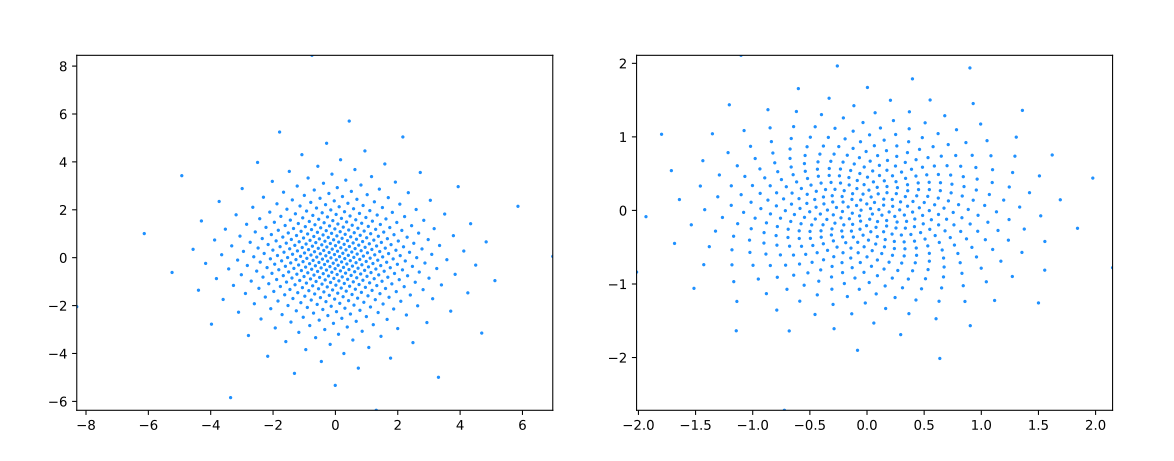
\includegraphics[width=0.48\textwidth]{fig1.png}
    \caption{(a) 500 Punkte mit einer logistischen Dichte auf der X- und Y-Achse (b) 500 Punkte standardnormalverteilt \eqref{eq:stdnormdensity}.}
    \label{bild:examplePlot}
\end{figure}


Bei einem Zufallsvektor $ (X_1, ..., X_n) \in \mathbb{R}^n$ wird die Inversionsmethode auf je eine Dimension angewandt 
und dann die folgende Zufallszahl generiert und dann rekursiv die nachfolgenden Dimensionen berechnet. Genauer bedeutet das, 
dass zuerst die Variable $X_n$ der höchsten Dimension berechnet wird. Danach wird $X_{n-1}$ mit der zugewiesenen Funktion 
berechnet, wobei $X_n$ als bedingte Verteilung mit eingerechnet wird.


\subsection{Hashtabelle}
Eine Hashtabelle ist eine Datenstruktur, die mithilfe einer Hashfunktion $H: V \rightarrow K$ einen Wert $v \in V$ 
auf den zugehörigen Schlüssel $k \in K$ ab. Die Werte werden dann in einem Array gespeichert, 
wobei der Schlüssel die Position angibt. Da es in der Praxis meistens mehr Werte als Stellen im Array gibt, treten 
allerdings Kollisionen auf. Diese können entweder dadurch gelöst werden, dass das Array pro Schlüssel eine verkettete 
Liste enthält. In diese werden dann die kollidierende Werte hintereinander geschrieben. Die zweite verbreitete Möglichkeit 
ist lineares Sondieren. Dabei wird der Wert immer an die nächste freie Stelle in der Hashtabelle, von seinem eigentlichem 
Platz aus gesehen, geschrieben.


\subsection{Inversion mit Hashing}
Um die Inversionsmethode zu beschleunigen, gibt es mehrere Möglichkeiten. Eine davon ist, 
eine Hashtabelle zu verwenden, indem die von Chen und Asau \cite{chen_asau-generating_random_variates-1974} erarbeitete 
Vorgehensweise verwendet wird. Um diese Methode zu verwenden, wird für $j \in [1, n]$ die Wahrscheinlichkeit $p_j$ als 
$p_j = P(X=v_y)$ definiert. Mithilfe einer uniformen Variablen $U \in [0, 1]$ wird die Zufallsvariable $X$ durch 
\begin{equation}
    F(v_{j-1}) < U \leq F(v_j)
    \label{eq:hash_ineq}
\end{equation}
berechnet, wobei $X = v_j$ ist. Diese Ungleichheit kann zwar ohne großen Aufwand berechnet werden, doch bei vielen $j$ 
läuft jede Generierung in $O(n)$. Mit dem Einsatz einer Hashtabelle, die wie eine Indextabelle agiert, kann jede 
Generierung in approximiert $O(1)$ laufen. Dafür wird aus den Werten $F(v_j)$ ein Wert
\begin{equation}
     I_j = \lfloor F(v_j) * d \rfloor + 1
     \label{eq:hash_I}
\end{equation}
berechnet. Dabei wird $d = 10^m$ so gewählt, dass $\mathrm{min}(I_j) = 1$ ist. Danach wird die Indextabelle $T(k),\, k \in [1,\, 
\mathrm{max}(I_j)]$ initialisiert. Dafür werden die $I_j$ als Indexliste verwendet. Für jedes $I_j$ wird $T(I_j)$ als das 
$k$ gesetzt, für das $I(k) = I(j)$ ist. Falls ein Element $I_k$ nicht in der Indexliste vorhanden ist, gilt $T(I_k) = T(I_{k+1})$. 

Nach diesen Vorberechnungen und Initialisierungen kann die Hashtabelle verwendet werden, um eine Zufallszahl $X$ zu berechnen. 
Dafür wird aus einer uniformen zufälligen Zahl $U\; I_U$ \eqref{eq:hash_I} und $i = T(I_U)$ berechnet. $i$ beschränkt 
damit die Teilmengen $F(v_j)$, die \eqref{eq:hash_ineq} erfüllen können. Die zu überprüfenden Teilmengen sind gegeben 
durch $\{F(v_i),\, \dots, \, F(v_{r-1})\}$, wobei $r$ die nächstgrößere Zahl ist, für die $I(i) \neq I(r)$ gilt. 
Für den Fall, dass $U > F(v_{r-1})$ ist, gilt bei Einsatz der Hashtabelle $T$ immer $U \leq F(v_r)$, da ansonsten nicht $i = T(I_U)$ 
gelten würde. Nachdem ein $v_j$ gefunden wurde, für das \eqref{eq:hash_ineq} erfüllt ist, wird $X$ auf $v_j$ gesetzt.

12 Jahre nach Chen und Asau's Ansatz wird in Devroye \cite{devroye-non_uniform_random_variate-1986} eine abgewandelte Methode 
vorgestellt. Dabei wird eine Hashtabelle der Größe $N$ erstellt, wobei $N$ die Anzahl der möglichen Werte angibt. An der $i$-ten 
Stelle in der Hashtabelle wird der Wert von $X$ mit $P(X) = p_X$ gespeichert, falls $U = \dfrac{i}{N},\, i \in [0,\, N)$ wäre. Nach 
dieser Initialiserung wird der Startindex $Z$, ab welchem eine Lösung zu finden ist, mit $Z = \lfloor N * U \rfloor$ berechnet. 
Mit $Z$ kann jetzt in der Hashtabelle ab diesem Index mit minimalem Aufwand eine Lösung der bekannten Formel \eqref{eq:hash_ineq} von Chen 
und Asau gesucht werden. 

\input{Einschränkungen}

\section{Vergleich}
\begin{figure}
    \centering
    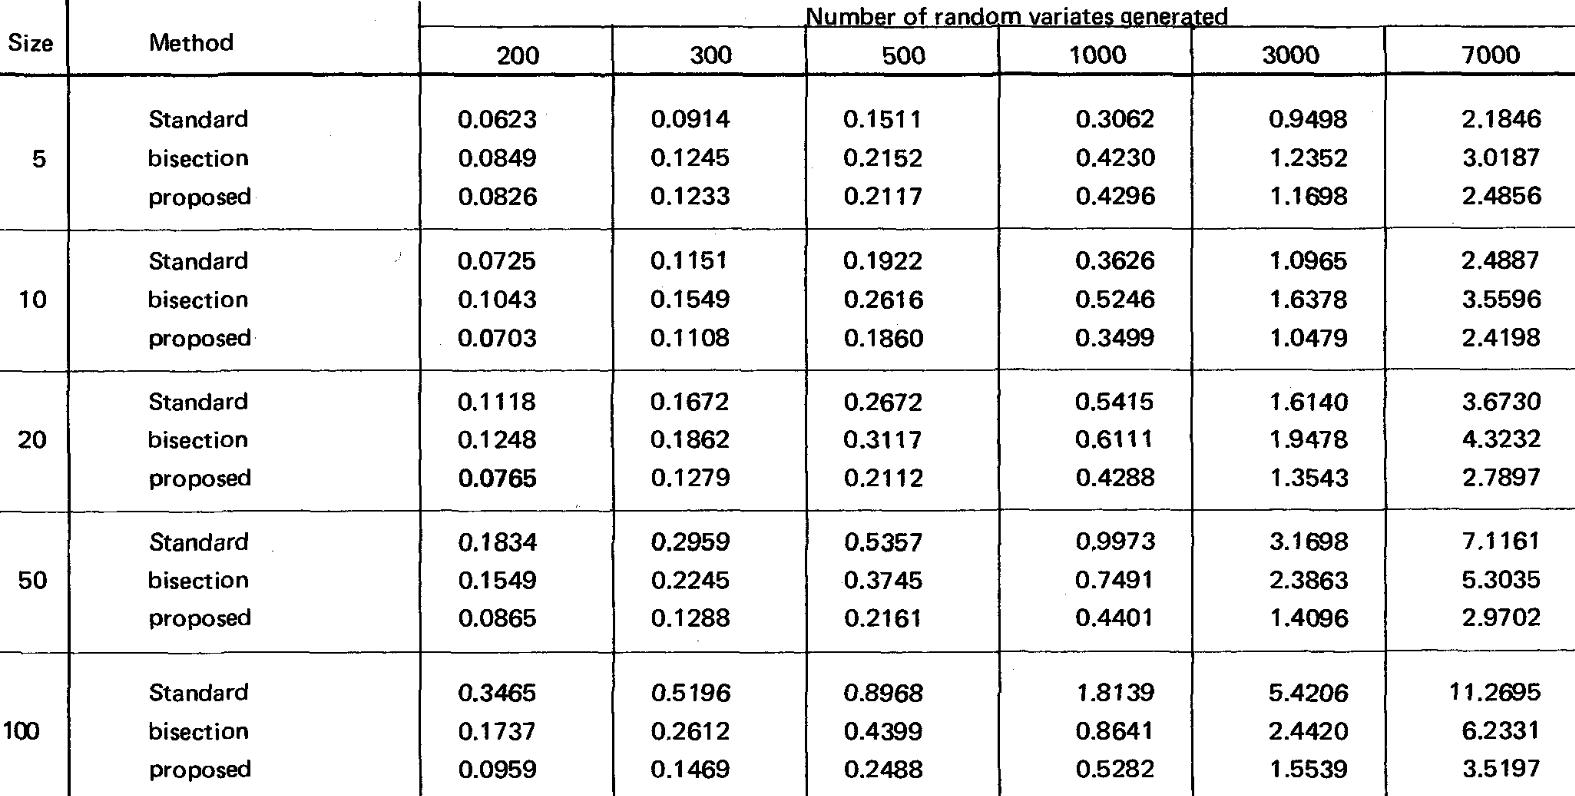
\includegraphics[width=0.48\textwidth]{Screenshots/chenAsauHashTableComp.png}
    \caption{Laufzeiten unterschiedlicher Algorithmen: Standard (\eqref{eq:hash_ineq} 
        wird trivial berechnet), Bisection (\eqref{eq:hash_ineq} wird mit einfacher 
        binarär Suche berechnet) und Proposed (die vorgestellte Methode mit 
        Indextabelle). Auszug aus Chen und Asau \cite{chen_asau-generating_random_variates-1974}.}
    \label{fig:computationTimeComp}
\end{figure}
Chen und Asau haben in ihrer Arbeit über die hash-basierte Inversionsmethode 
gezeigt, dass ihre Methode für große Zahlen um eine Magnitude schneller ist, 
als triviale Methoden. Durch den Einsatz der Hashtabelle werden, anstelle von 
$O(n)$ Berechnungen wie bei der trivialsten Methode lineare Suche oder $O(\log
(n))$ Berechnungen bei binärer Suche, bei gut gewählter Größe der Hashtabelle 
nur noch $O(1)$ Berechnungen je Zufallsvariable durchgeführt. Diese Verbesserung 
hängt mit der 
Eigenschaft von Arrays und Hashtabellen zusammen, auf jedes Element in $O(1)$ 
zugreifen zu können. Deshalb kann die hashbasierte Inversionsmethode ihre 
Stärken erst bei vielen zu überprüfenden Intervallen, und damit Einträgen in 
der Tabelle, ausspielen. In Chen und Asau's Tests sieht man, das für wenige 
Intervalle ($5$) die Hashtabelle langsamer ist als triviales Testen der 
Ungleichungen. Mit $100$ Einträgen ist die vorgestellte Methode aber schon mehr 
als $3$-mal so schnell wie herkömmliche Verfahren. Das liegt daran, dass bei 
wenigen Intervallen die Initialisierung der Hashtabelle einen sog. Overhead 
erschafft, da der Aufwand, sie mit Werten zu befüllen und alle Möglichkeiten 
vorher zu berechnen, nicht durch viele Zugriffe wieder gutgemacht wird.

Wie in der Einleitung benannt, gibt es noch die Möglichkeit, Huffman-Bäume 
einzusetzen. Diese kodieren Werte nach ihrer Häufigkeit, wodurch häufig 
vorkommende Werte kürzer dargestellt werden und dadurch weniger Platz, verbrauchen. 
Diese Bäume können auch traversiert werden, wobei auch hier der kürzere Weg für 
häufigere Werte von Vorteil ist. Es ist möglich, einen solchen Baum abzuwandeln, 
damit er sinnvoll in der Partialsummenberechnung eingesetzt werden kann. Dadurch 
ergeben sich optimale Laufzeiten, die durch konstante Werte je nach Implementierung 
sogar besser als jene einer Hashtabelle sein können. In dieser Arbeit werden 
allerdings keine Vergleiche gezeigt, da die Implementierung eines Huffman-Baumes 
über den Rahmen dieser Ausarbeitung hinausgehen würde.

Durch die Hashtabelle werden bei sehr großen Mengen an Zufallsvariablen viele 
komplizierte Berechnungen gespart, da nur bei der Initialisierung die 
möglicherweise aufwändige Invertierung berechnet wird. Durch das Zusammenfallen 
von Werten durch nur endlich viele Einträge in der Hashtabelle, eignet sich die 
hashbasierte Inversion allerdings nur, wenn die Berechnung und Auswertung der 
Dichtefunktion sehr aufwändig ist und man nicht die Ressourcen oder Zeit besitzt, 
diese für jeden Wert auszuführen.



\section{Implementation}
\label{impl}
\begin{figure*}[htb!]
    \centering
    \begin{subfigure}[b]{.3\textwidth}
        \centering
        \includegraphics[width=\textwidth]{pdf_plots/idf2_log-sin_ir500c-RND.pdf}
        \caption{Eingabewerte zufällig generiert mit \code{random}}
        \label{fig:logsin_random}
    \end{subfigure}
    \hfill
    \begin{subfigure}[b]{.3\textwidth}
        \centering
        \includegraphics[width=\textwidth]{pdf_plots/idf2_log-sin_iu500c-GRS.pdf}
        \caption{Eingabewerte aus einer Goldenen Schnitt Sequenz}
        \label{fig:logsin_uniform}
    \end{subfigure}
    \caption{$500$ Punkte mit einer logistischen Dichte auf der X- und einer sinusoiden auf der Y-Achse}
    \label{fig:rand_vs_uniform}
\end{figure*}


Um einen Eindruck der hashbasierten Inversionsmethode und ihrer Arbeitsweise zu bekommen, 
wird jetzt eine konkrete Implementierung dieser angesprochen und Ergebnisse bei 
unterschiedlichen Eingaben gezeigt. Geschrieben wurde das Programm in Python mithilfe der 
Pakete \textit{numpy} und \textit{matplotlib}.

Schretter \cite{schretter-golden_ratio_sequences-2012} stellt am Ende der Arbeit eine 
C++-Methode zur Generierung einer zweidimensionalen Goldenen-Schnitt-Sequenz zur Verfügung. 
Diese Methode wurde in ein Python-Script übertragen und alle, in diesem Kapitel erwähnte, zufällige, uniformen
Variablen $U$ werden mit diesem Script generiert.

Zum Testen der vorgestellten Methode wurde das Konzept von Chen und Asau \cite{chen_asau-generating_random_variates-1974} 
implementiert. Dabei wurde kein großer Wert auf optimale Laufzeiten gelegt, sondern darauf, eine Demonstration 
des Verfahrens geben zu können.

% TODO
% Ergebnisse bei unterschiedlichen Werten auswerten nicht nur im Bild
\dots




\section{Zusammenfassung}

\begin{frame}{Kurz \& Knapp}    
    \begin{itemize}
        \item Schnelle Generierung von großen Datenmengen
        \item<2-> Beibehaltung aller Eigenschaften der ursprünglichen Funktion
        \item<3-> einfaches Prinzip
    \end{itemize}
\end{frame}

\begin{frame}{Verbesserungsmöglichkeit}   
    \begin{itemize}
        \item\textbf{Problem:} Funktion mit sehr hoher Dichte an wenigen Stellen, sonst nur geringe Dichte.
        \begin{itemize}[label=$\rightarrow$]
            \item<2-> Dort fallen alle Punkte zusammen.
            \item<3-> Hohe Ungenauigkeit an wichtigen Stellen.
        \end{itemize}
        \item<4->\textbf{Lösung:} Hashtabelle nicht gleichmäßig populieren, sondern für diese 
        Stellen höhere Genauigkeit durch mehr Einträge ermöglichen.
        \item<5->\textbf{Allerdings:} stark erhöhter Initialisierungsaufwand
    \end{itemize} 
\end{frame}

% Code
%\section{Code}

\begin{algorithm}
    \caption{Implementation of the hash-based inversion method (Part 1)}
    \label{alg:inv_hash}
    \begin{algorithmic}
        
        \Input
        \Desc{N}{Size of the hash table}
        \Desc{f\_inv}{inverse function for this table}
        \EndInput
        \Function{\_\_init\_\_}{$self$, N, $f\_inv$}
            \State $self.T \gets [\,]$ \Comment{hash table}
            \State $self.PS \gets$ np.array$([\,])$ \Comment{list of partial sums}
            \State $self.N \gets$ N
            \State $self.f\_inv \gets$
            \For{$i$ in range$(0, self.N)$}
                \State $self.T.$append$(self.f\_inv(\frac{i}{self.N}))$
            \EndFor
            \State $self.T \gets$ np.array$(self.T)$
        \EndFunction
        \State
        
        \Input
        \Desc{f}{inverse function of $self.f\_inv$}
        \Desc{max}{amount of partial sums}
        \EndInput
        \Function{setup\_partial\_sums\_uniform}{$self$, f, max}
            \State $ps \gets [\,]$
            \State $i \gets 0.0$
            \State $step \gets \frac{\textrm{max}}{self.N}$
            \While{$i < \textrm{max}$}
                \If{$i == 0.0$}
                    \State $ps.\textrm{append}(\textrm{f}(0))$
                \Else
                    \State $ps.\textrm{append}(ps[-1] + \textrm{f}(i))$
                \EndIf
                \State $i \gets i + step$
            \EndWhile
            \State $self.PS \gets \textrm{np.array}(ps)$
        \EndFunction
        \State

        \algstore{bkbreak}
    \end{algorithmic}
\end{algorithm}

\begin{algorithm}
    \caption{Implementation of the hash-based inversion method (Part 2)}
    \begin{algorithmic}
        \algrestore{bkbreak}
        \Input
        \Desc{U}{random variate}
        \EndInput
        \Output
        \Desc{h}{hashed value of $U$}
        \EndOutput
        \Function{hash}{$self$, U}
            \State\Return $\lfloor self.N * \textrm{U} \rfloor$
        \EndFunction
        \State


        \Input
        \Desc{U}{random variate}
        \EndInput
        \Output
        \Desc{X}{from hash table calculated value corresponding to $U$, so that $\mathrm{f^{-1}}(U) = X$}
        \EndOutput
        \Function{search\_single}{$self$, U}
            \State $Z \gets self.hash(\textrm{U})$
            \While{$self.PS[Z] \le \textrm{U}$}
                $Z \gets Z + 1$
            \EndWhile
            \State\Return $self.T[Z]$
        \EndFunction
    \end{algorithmic}
\end{algorithm}


% Literaturverzeichnis in Literatur.bib
\bibliographystyle{plain}
\bibliography{Literatur}
\end{document}